\documentclass[10pt,twocolumn]{article}
\usepackage{geometry}
\geometry{verbose,headsep=3cm,tmargin=2.5cm,bmargin=2.5cm,lmargin=2.0cm,rmargin=2.0cm}
\usepackage{graphicx}
\usepackage{xcolor}
\usepackage[font=small]{caption}
\usepackage{amsmath,amssymb,latexsym}
\usepackage{marvosym}
\usepackage{url}
\usepackage{lipsum}
\usepackage{bm}
\usepackage{float}
\usepackage[english]{babel}
\usepackage{hyperref}
\usepackage{epsf}
\usepackage{float}
\usepackage{mathpazo}
\usepackage{pifont}
\usepackage{wrapfig}
\usepackage{multicol}
\usepackage{enumitem}
\usepackage{xcolor}
\usepackage{framed}
\usepackage[utf8]{inputenc}
\graphicspath{{DWGs/}}
\usepackage{framed}
\usepackage{textcomp}
\usepackage{braket}
\newcommand{\highlight}[1]{%
  \colorbox{orange!50}{$\displaystyle#1$}}
% Default fixed font does not support bold face
\DeclareFixedFont{\ttb}{T1}{txtt}{bx}{n}{10} % for bold
\DeclareFixedFont{\ttm}{T1}{txtt}{m}{n}{10}  % for normal

% Custom colors
\usepackage{color}
\definecolor{deepblue}{rgb}{0,0,0.5}
\definecolor{deepred}{rgb}{0.6,0,0}
\definecolor{deepgreen}{rgb}{0,0.5,0}

\usepackage{listings}

% Python style for highlighting
\newcommand\pythonstyle{\lstset{
language=Python,
basicstyle=\ttm,
otherkeywords={self},             % Add keywords here
keywordstyle=\ttb\color{deepblue},
emph={MyClass,__init__},          % Custom highlighting
emphstyle=\ttb\color{deepred},    % Custom highlighting style
stringstyle=\color{deepgreen},
frame=tb,                         % Any extra options here
showstringspaces=false            % 
}}


% Python environment
\lstnewenvironment{python}[1][]
{
\pythonstyle
\lstset{#1}
}
{}

% Python for external files
\newcommand\pythonexternal[2][]{{
\pythonstyle
\lstinputlisting[#1]{#2}}}

% Python for inline
\newcommand\pythoninline[1]{{\pythonstyle\lstinline!#1!}}
% Document font:
\usepackage{charter}

\begin{document}

%%% HEADER --------------------------------------------------------------
% ------------------------------------------------------------------------

\twocolumn[{
\begin{@twocolumnfalse}

  \begin{center}
%\textcolor{lgray}
    \vskip-5em

    \hfill
    \fontsize{10}{10}\selectfont {\textit{Bruxelles, January 2019}}
    \vskip2ex
	\vspace{5ex}
    \fontsize{20}{10}\selectfont {The linear algebra of Principal Component Analysis}
      \vspace{1ex}
      
      \fontsize{16}{10}\selectfont {(with some Python)}
  \noindent%
    
\vskip1ex

{\rule{\textwidth}{0.5pt}}

  \end{center}
  
\vspace{8mm}

\end{@twocolumnfalse}
}]

%%% HEADER END -----------------------------------------------------------
% ------------------------------------------------------------------------

\vspace{10mm}

\setlength{\parindent}{0cm}

\fontsize{14}{10}\selectfont {Kamila Zdybał}

\vspace{2mm}

\fontsize{8}{10}\selectfont {\textit{Université libre de Bruxelles, kamila.zdybal@ulb.ac.be}}

\fontsize{8}{10}\selectfont {\textit{camillejr.github.io/science-docs, kamila.zdybal@gmail.com}}

\section*{Preface}

These are notes on \textbf{Principal Component Analysis} (PCA), a dimensionality reduction technique in which a large data set is reduced to maintain only the directions of the largest variance.

\,\,

These notes are in a way a tutorial on PCA with a deeper focus on linear algebra and statistics aspects that govern this method, compared to other PCA tutorials that I have so far found on the web. I have an aim that the reader will both gain a deep and intuitive understanding as well as an appreciation for PCA after going through these notes. This requires a deep and intuitive understanding of several linear algebra concepts such as the eigendecomposition or matrix operations. 

\,\,

Some initial level of linear algebra knowledge and intuition is hence required.
I highly recommend a very pleasant to watch course by 3Blue1Brown YouTube channel, which, to my belief, will be everything you need to master about linear algebra to gain a great intuition behind PCA.

\,\,

This document is still in preparation. Please feel free to contact me with any suggestions, corrections or comments.

\section*{Keywords}

\textit{principal component analysis, data reduction, dimensionality reduction, linear algebra, MATLAB\textregistered, Python}

\tableofcontents

\section{Nomenclature}

\begin{tabular}{ll}
    $\bm{A}$ & is a matrix \\
    $A_{:,j}$ & is a vector formed by the $j^{th}$ column of a matrix $\bm{A}$, \\
    & it is equivalent to  $\bm{A}(:,j)$ \\
    $A_{i,:}$ & is a vector formed by the $i^{th}$ row of a matrix $\bm{A}$, \\
    & it is equivalent to  $\bm{A}(i,:)$ \\
    $a_{i,j}$ & is an element from $i^{th}$ row and $j^{th}$ column of a matrix $\bm{A}$, \\ 
    & it is equivalent to  $\bm{A}(i,j)$ \\
\end{tabular}

\section{Motivation for data reduction}

To motivate why studying techniques such as PCA and learning to apply them on real data sets is important, there are several questions which stimulated the development of data reduction and data decomposition techniques:

\begin{enumerate}
\item Can we send less data but preserve maximum information contained by the data (data compression)?

\item Can we predict what the outcome of another observation will be?

\item Can we build a model in a purely data-driven way - based on data that we have collected (e.g. from experiments or numerics)?

\item Can we make sense of a large, multi-dimensional data set (which cannot be plotted graphically)?

\item Can we extract low-dimensional features that underlay the data?
\end{enumerate}

\section{Data sets for PCA}

For the rest of this document, we assume that the data set for performing PCA is structured as follows: each column represents one variable $V_j$, where $j \in \braket{1, Q}$, and the rows correspond to variable observations $O_i$, where $i \in \braket{1, n}$, (e.g. at different positions in space, or in time). The raw data matrix $\bm{X}$ is size $(n \times Q)$.

\begin{figure}[H]
\centering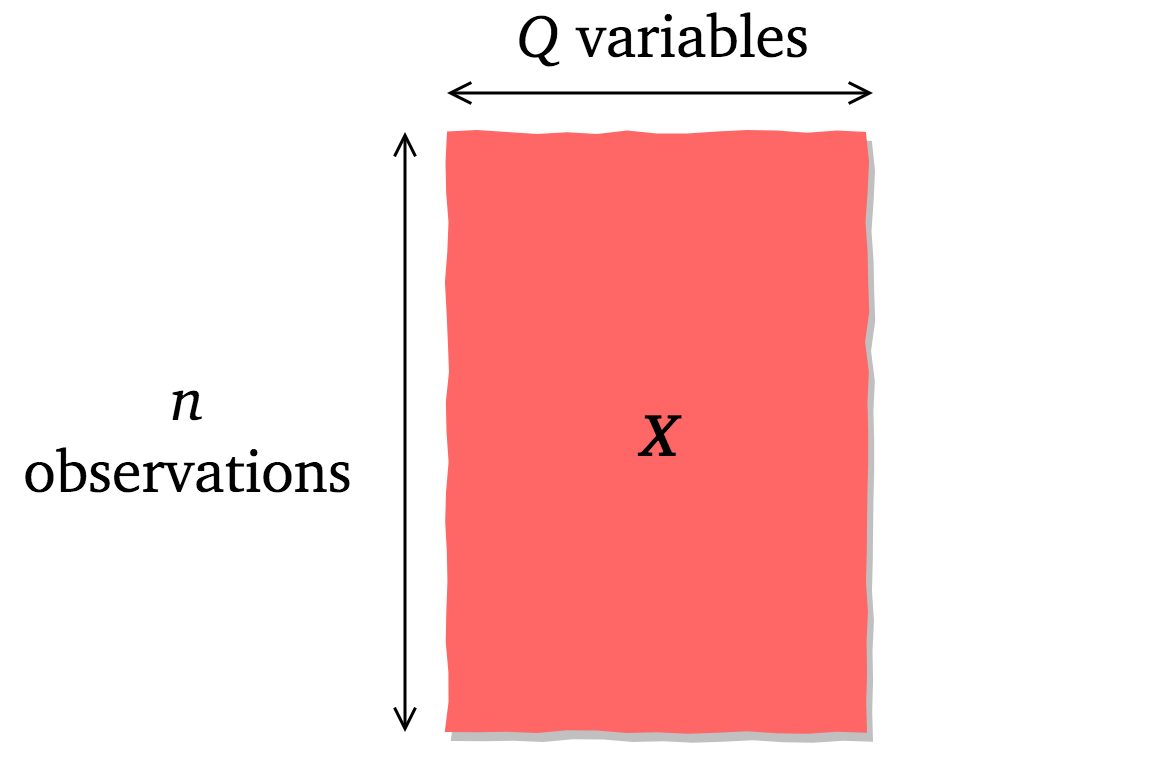
\includegraphics[width=5cm]{data-set-PCA.png}
\caption{Data matrix for PCA.}
\label{fig:data-matrix}
\end{figure}

This is also the data format that is needed for the MATLAB\textregistered \, command \texttt{pca}. From the documentation \cite{Matlab-pca}:


\begin{framed}
\texttt{pca(X)}
\,\,
Rows of X correspond to observations and columns correspond to variables.
\end{framed}

\section{Data pre-processing}

In data science we are typically given a raw data set which is not centered and not scaled. 

Data centering allows to look at it as variations from some center. Typically we might center each variable by subtracting the mean of this variable's observations (realizations) - we would then look at the data as variations from the mean. This would substitute the original data set with:

\begin{equation}
\bm{X'} = \bm{X} - \text{mean}(\bm{X})
\end{equation}

Such centering will shift the "cloud" of data points (which in general is multi-dimensional) to the origin. However, other values for centering are possible.

Scaling, on the other hand, allow us to cancel the effect of unit that a variable might have and treat all variables with equal importance. 

\begin{equation}
\bm{X''} = \bm{X'}\bm{D}^{-1}
\end{equation}

In the above equation, the matrix $\bm{D}$ is a diagonal matrix whose entries are the corresponding scalings. Hence, every column of the matrix $\bm{X'}$ gets divided by a corresponding scale from the diagonal of the matrix $\bm{D}$.

You might for instance think about a set of variables from a single experiment, representing temperature in the units of $[K]$ and range from 300-1500 $K$ and associated pressures in the units of $[atm]$ which range from 1-1.1 $atm$. If we did not scale the data, the largest "spread" or the variance would be found in temperature, since on purely numerical  grounds, the range 300-1500 is more significant than the range 1-1.1.

For simplicity, for the rest of this document we assume that $\bm{X}$ represents pre-processed data (in place of $\bm{X'}$ or $\bm{X''}$).

\section{Covariance matrix}

\subsection{Construction}

The starting point for performing PCA is to compute a \textit{covariance matrix} from the data set. The covariance matrix is given by:

\begin{equation}
\bm{S} = \frac{1}{n-1} \bm{X}^T \bm{X}
\end{equation}

and is therefore size $(Q \times Q)$.

We will start by exploring the meaning of $\bm{X}^T \bm{X}$. Let's look at the graphical representation of this matrix multiplication in Figure \ref{fig:covariance-matrix}.



Any given column, say $p$ or $k$, of the data matrix $\bm{X}$ represents all measurements of a single variable $V_p$ (or $V_k$) and can be viewed as a single $n$-dimensional vector. The same can be said about any row of a matrix $\bm{X}^T$.

\begin{figure}[H]
\centering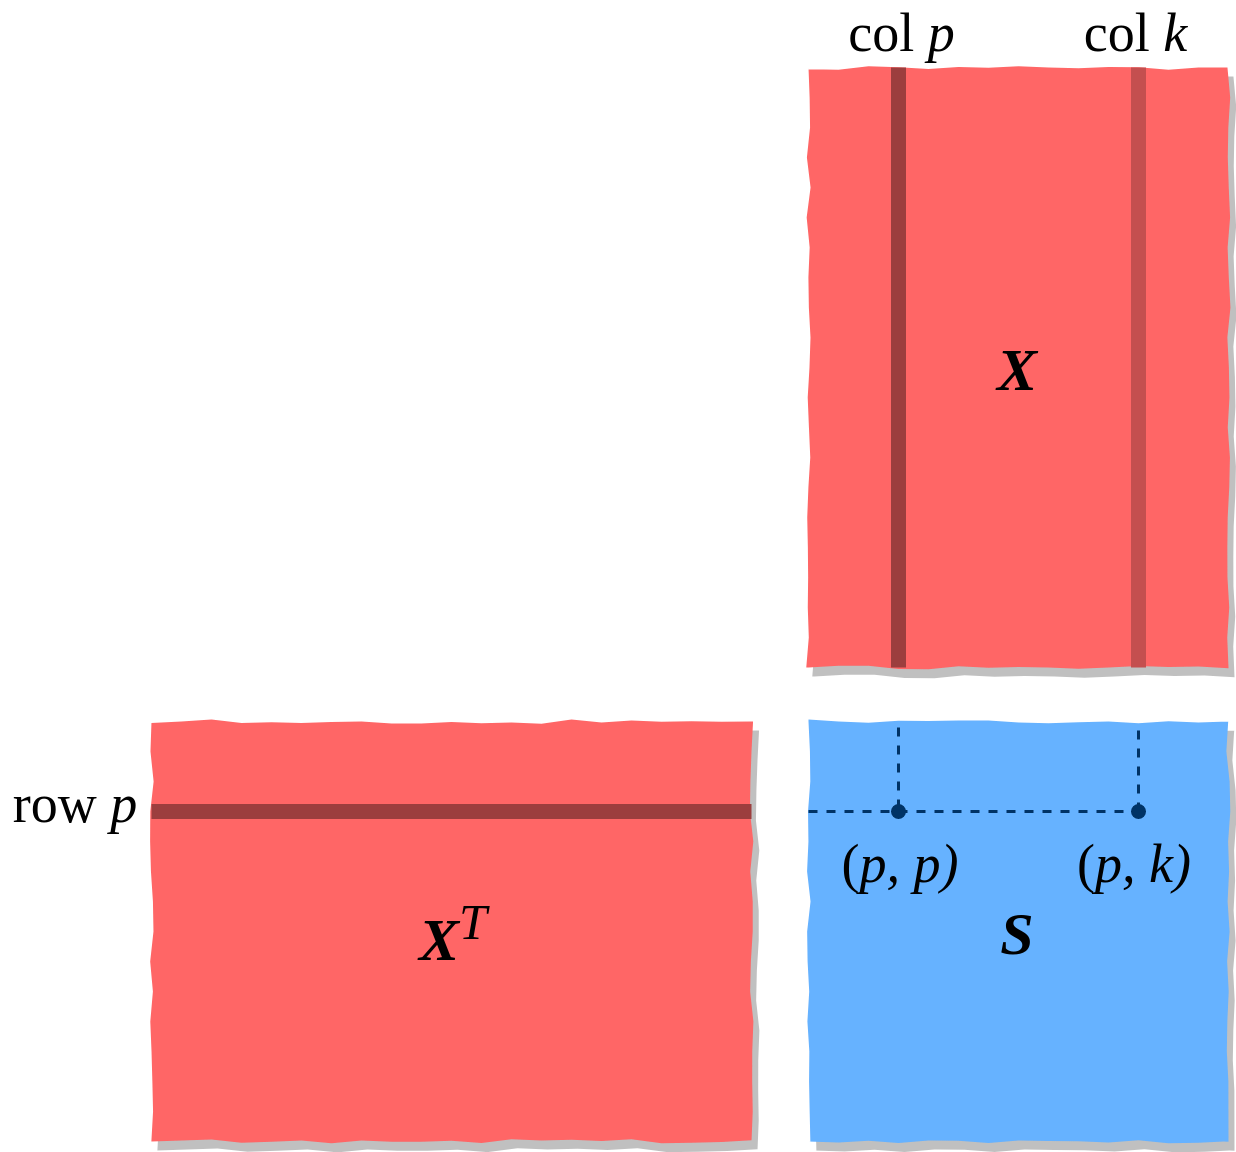
\includegraphics[width=7.5cm]{cov-matrix.png}
\caption{Covariance matrix $\bm{S}$ graphical interpretation.}
\label{fig:covariance-matrix}
\end{figure}

Notice that an element at position $(p,k)$ inside the matrix $\bm{S}$ has the interpretation of a dot product between a vector formed by the $p$-th row of a matrix $\bm{X}^T$ and a $k$-th column of a matrix $\bm{X}$. There is also the $\frac{1}{n-1}$ factor out front to which we come back in the Appendix \ref{app:B}.

\begin{equation}
s(p,k) = \frac{1}{n-1} \text{dot}( \bm{X}^T(p, :), \bm{X}(:,k))
\end{equation}

In a special case, where we multiply the row $p$ with the column $p$, we get a dot product of a vector with itself.

\begin{equation}
s(p,p) = \frac{1}{n-1} \text{dot}( \bm{X}^T(p, :), \bm{X}(:,p))
\end{equation}

In general, the dot product between two vectors $x$ and $y$ represents how much vector $x$ lays in the direction of vector $y$ (and vice versa) - and it is zero when two vectors are perpendicular to each other. This intuition can be carried to our covariance matrix $\bm{S}$. If any off-diagonal element is non-zero, say element at position $(p,k)$ this means that some information about variable $V_p$ is carried by a variable $V_k$ (and vice versa).

In other words, every element in the covariance matrix is computed as:

\begin{equation}
s(i,j) = \frac{1}{n-1} \sum\limits_{k=1}^n V_i(k) V_j(k)
\end{equation}

\subsection{Properties}

The covariance matrix is a very special matrix and it is worth pointing out some of its interesting properties that the Principal Component Analysis makes use of.

First of all, a matrix constructed as: $\bm{S} = \bm{C}^T \bm{C}$ (where $\bm{C}$ is any real matrix) is square and symmetric (the reason for this is easy to see from Figure \ref{fig:covariance-matrix}). Apart from that, the eigenvalues of such matrix are real and all are at least non-negative - such matrix is called a \textit{positive semidefinite} matrix. In a practical case that we are most interested in, this matrix has got only positive eigenvalues and we call it a \textit{positive definite} matrix.

Another important property is that the eigenvectors of the covariance matrix are orthogonal, which is a very special thing indeed. You may already see some interesting uses for such eigenvectors. One of which could be: they can form a new coordinate system, in other words: a \textit{basis}. The question thus remains: can such basis be any interesting basis?

\section{PCA workflow}

As you may have already anticipated, the next step in PCA is to perform the eigendecomposition of the covariance matrix:

\begin{equation} \label{eq:eig-dec}
\text{eig}(\bm{S}) = [\bm{A}, \bm{\Lambda}]
\end{equation}

The matrix $\bm{A}$ is a matrix of eigenvectors and it is size $(Q \times Q)$. Each eigenvector is called a \textit{principal component} (PC). The principal components are orthogonal to each other, and therefore the following important property holds: $\bm{A}^T = \bm{A}^{-1}$ (proof\footnote{Proof: for orthogonal columns of $\bm{A}$ we have $\bm{A}^T \bm{A} = \bm{I}$ Multiplying both sides by $\bm{A}^{-1}$ we get $(\bm{A}^T \bm{A}) \bm{A}^{-1}= \bm{I}\bm{A}^{-1}$. Since matrix multiplication is associative, we may also perform: $\bm{A}^T (\bm{A} \bm{A}^{-1}) = \bm{A}^{-1}$. From definition of an inverse matrix,  $\bm{A} \bm{A}^{-1} = \bm{I}$, hence: $\bm{A}^T = \bm{A}^{-1}$.}).

The diagonal matrix $\bm{\Lambda}$ of size $(Q \times Q)$ is a matrix of the corresponding eigenvalues.

Given the eigendecomposition of matrix $\bm{S}$, we may state that: $\bm{S} = \bm{A} \bm{\Lambda} \bm{A}^T$.

The principal components form a new basis in which we can represent our data set. We perform a transformation of the original data matrix $\bm{X}$ from the original space to the new space represented by the PCs. This transformation is achieved by the following multiplication:

\begin{equation} \label{eq:data-transform}
\bm{Z} = \bm{X} \bm{A}
\end{equation}

\begin{figure}[H]
\centering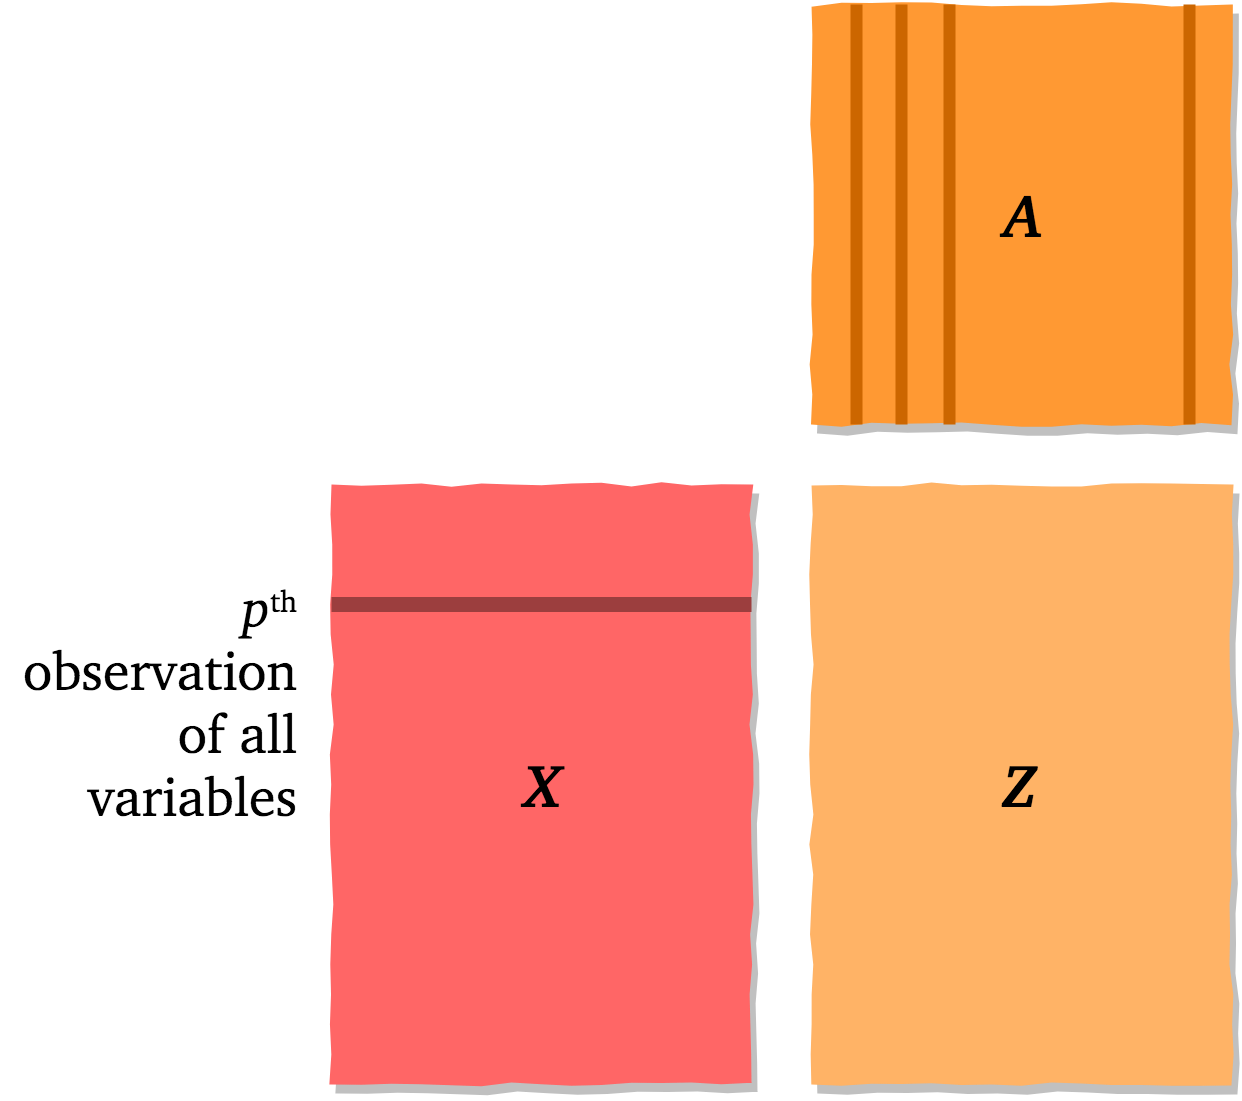
\includegraphics[width=6cm]{data-transformation.png}
\caption{Data transformation to a new basis.}
\label{fig:data-transformation}
\end{figure}

The new matrix $\bm{Z}$ is still our dataset $\bm{X}$ but represented in the basis associated with the matrix $\bm{A}$. It is also called the \textit{PC-scores} matrix, since one may think of every element in this matrix as the "score" that the corresponding element in $\bm{X}$ gets when represented in the new coordinate system after transformation.




In the matrix multiplication from eq.(\ref{eq:data-transform}), every variable vector inside $\bm{X}$ gets transformed by the transformation matrix $\bm{A}$ and attains new scores in the basis associated with $\bm{A}$. The new representation of the old variable is now kept in the matrix $\bm{Z}$.



We now approach the dimensionality reduction but first let's obtain the original data set back, given the PC-scores and the transformation matrix:

\begin{equation}
\bm{X} = \bm{Z} \bm{A}^T
\end{equation}

The above equation is our route back to obtain the original data set in which the PC-scores are projected on the basis associated with a transposed eigenvectors matrix $\bm{A}$ (recall that $\bm{A}^T = \bm{A}^{-1}$).

\begin{wrapfigure}{R}{0.2\textwidth}
\centering
\includegraphics[width=3cm]{new-basis.png}
\caption{Eigenvalues of the covariance matrix form a new basis.}
\label{fig:new-basis}
\end{wrapfigure}

Suppose that we would like to find the approximation of the data matrix $\bm{X}$ with only $q$ principal components (we project the PC-scores onto only $q$ out of $Q$ principal components).

We shrink the transformation matrix $\bm{A}$ to be of size $(Q \times q)$ (we only keep $q$ principal components). To match the matrix sizes we also need to shrink in size the PC-scores matrix which originally is size $(n \times Q)$ - the same size as the data matrix $\bm{X}$. We will denote these truncated matrices $\bm{A_q}$ and $\bm{Z_q}$ respectively.

Projecting $\bm{Z_q}$ onto the basis $\bm{A_q}^T$ will result in an an approximation of the original data set:

\begin{equation}
\bm{X_q} = \bm{Z_q} \bm{A_q}^T
\end{equation}


\begin{figure}[H]
\centering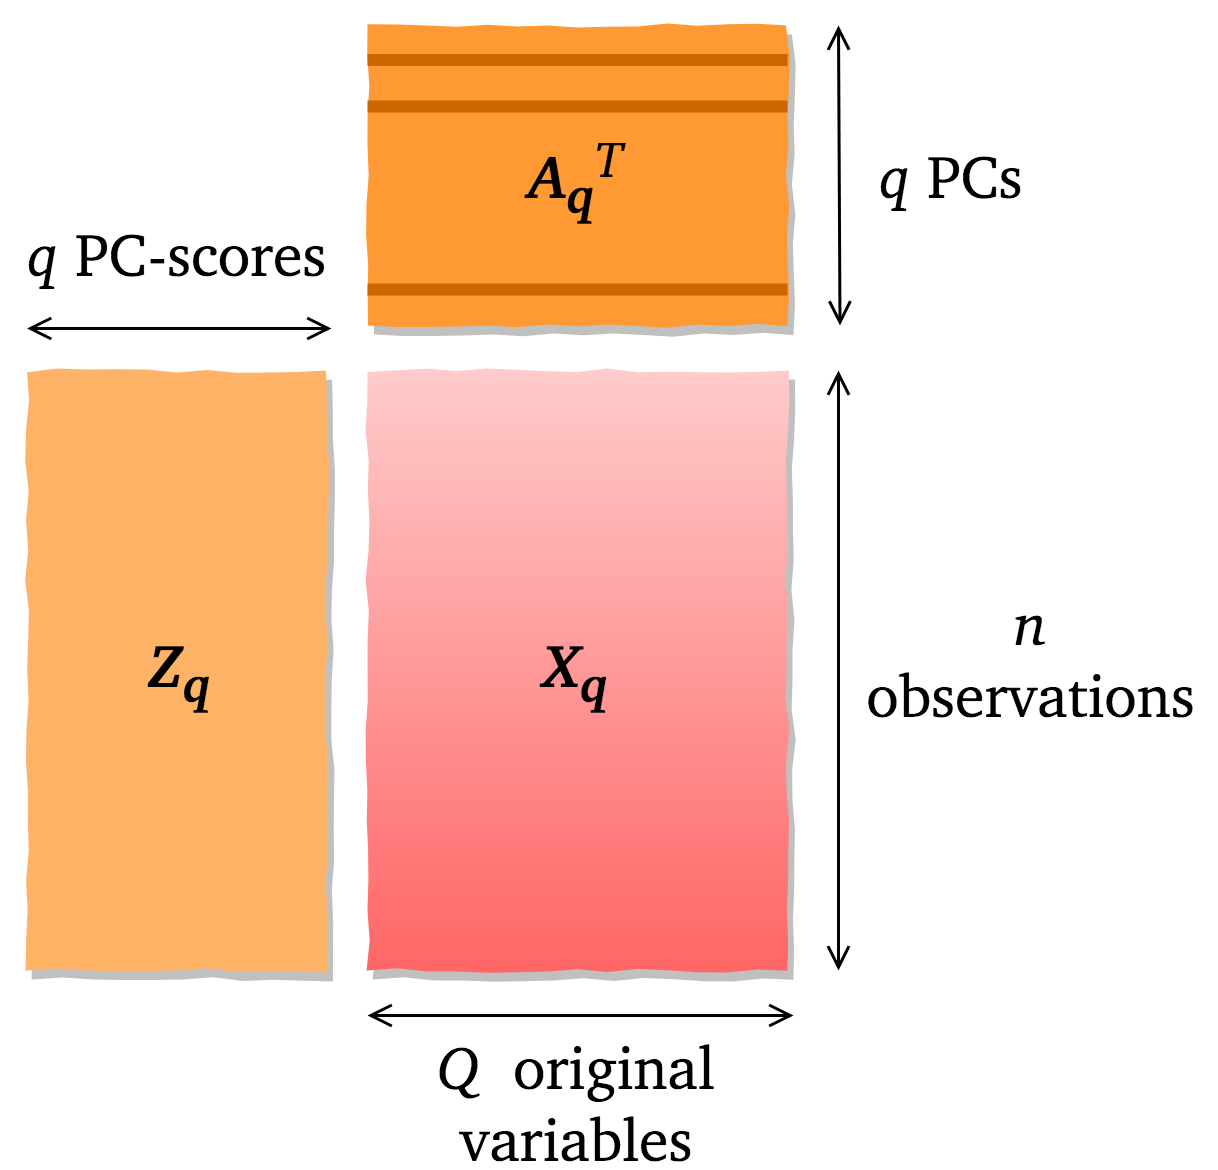
\includegraphics[width=5.5cm]{data-approx.png}
\caption{Data approximation with $q$-PCs.}
\label{fig:data-approx}
\end{figure}




\section{Why does it need to be eigenvectors?}

In this section we come back to equation (\ref{eq:eig-dec}) and answer the question: why are principal components the eigenvectors of a covariance matrix? If you are new to PCA, this indeed might seem like a not-related-to-anything thing to do. So why is it eigenvectors? And why does it need to be eigenvectors of this special matrix called covariance matrix?

To begin the understanding, let's look back at Figure \ref{fig:PC-scores}. What we want to achieve with PCA is to diagonalize the new covariance matrix. And we already have produced one diagonal matrix even before computing PC-scores - it was the matrix of eigenvalues $\bm{\Lambda}$.


\newpage

\section{PCA Python example}

We will now go on to visualizing on an artificial 2D data set every step of PCA. We will use the \pythoninline{PCA} function from a Python library \pythoninline{sklearn.decompositions}. The full code can be accessed in the GitHub repository. Here, we will only recall elements of that code to explain what is happening.

We create the \pythoninline{Dataset} (the equivalent of $\bm{X}$) as follows:

\begin{python}
import numpy as np
Np = 100
x = np.linspace(3, 6, Np)
y = 0.8*x + 1*np.random.rand(Np)
Dataset = np.column_stack((x, y))
\end{python}

Let's assume that the first column of this data set are realizations of the first variable $x$ and the second column are realizations of the second variable $y$.

The two variables $x$ and $y$ span two dimensional space but the data set exhibits a low-dimensional structure which is easily visible to the eye just by looking at the Figure \ref{fig:python-raw-data}. We already see that the data seems to be spread along some linear function. Perhaps changing the basis to a basis associated with this linear function will be a more effective representation by our data set? Note here also, that for multidimensional data sets "seeing" such data structures is no longer possible (as it still is in 2-D or 3D). We need to rely on the dimensionality reduction technique that we chose to find this low-dimensional structure for us.

\begin{figure}[H]
\centering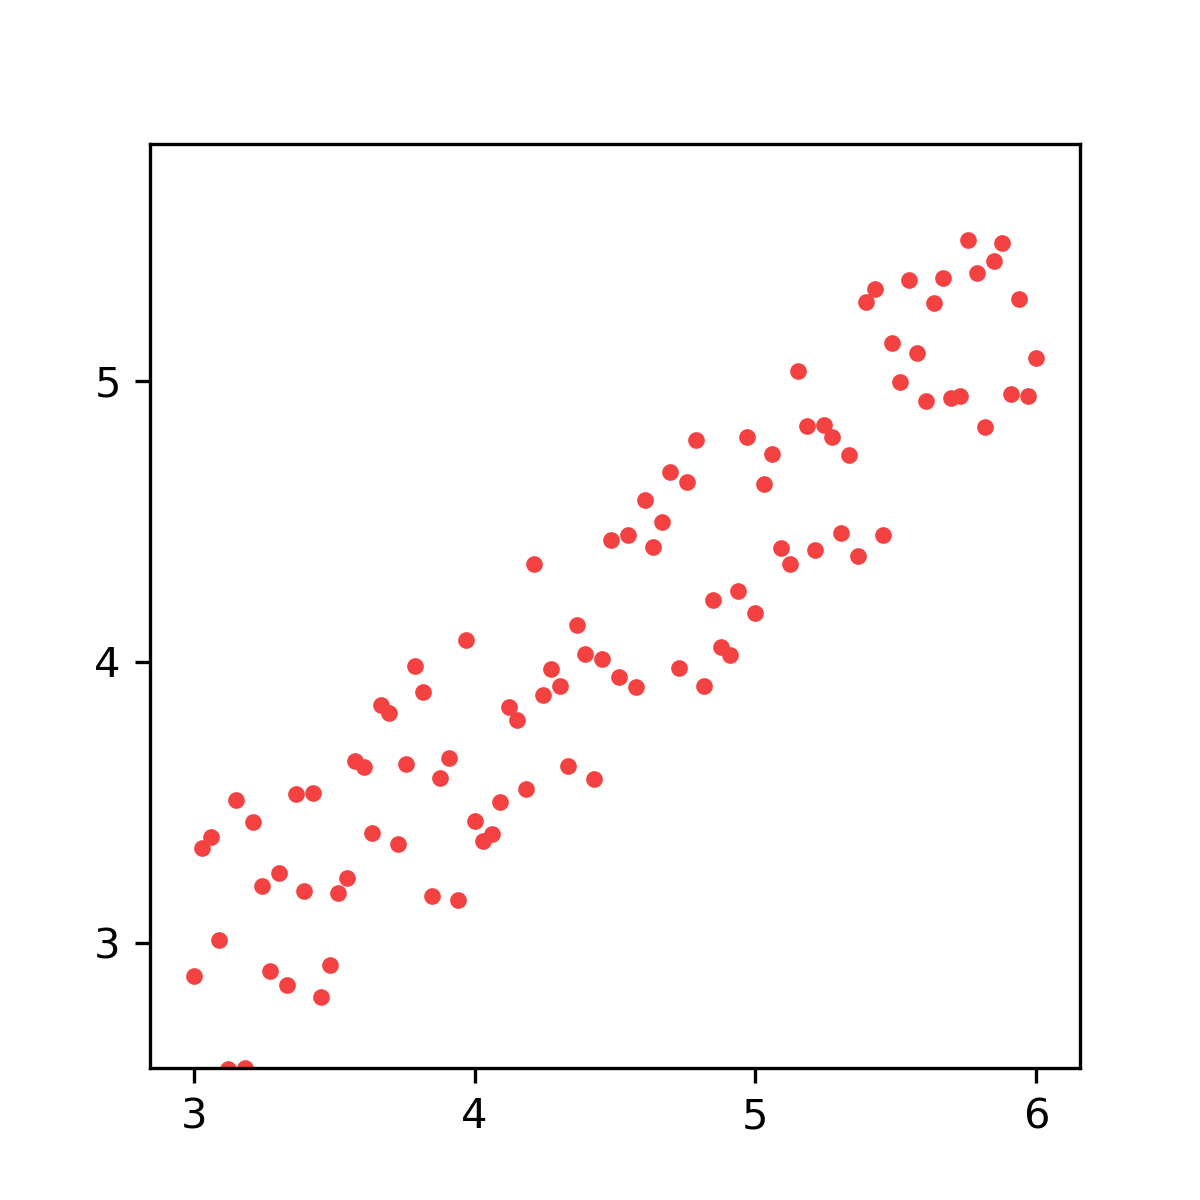
\includegraphics[width=7cm]{python-raw-data.png}
\caption{Raw data set.}
\label{fig:python-raw-data}
\end{figure}

We center the dataset, which simply moves the center of the cloud of points to the origin of the coordinate system. If necessary, data set would also be scaled to allow for even comparison of the two variables.

\begin{figure}[H]
\centering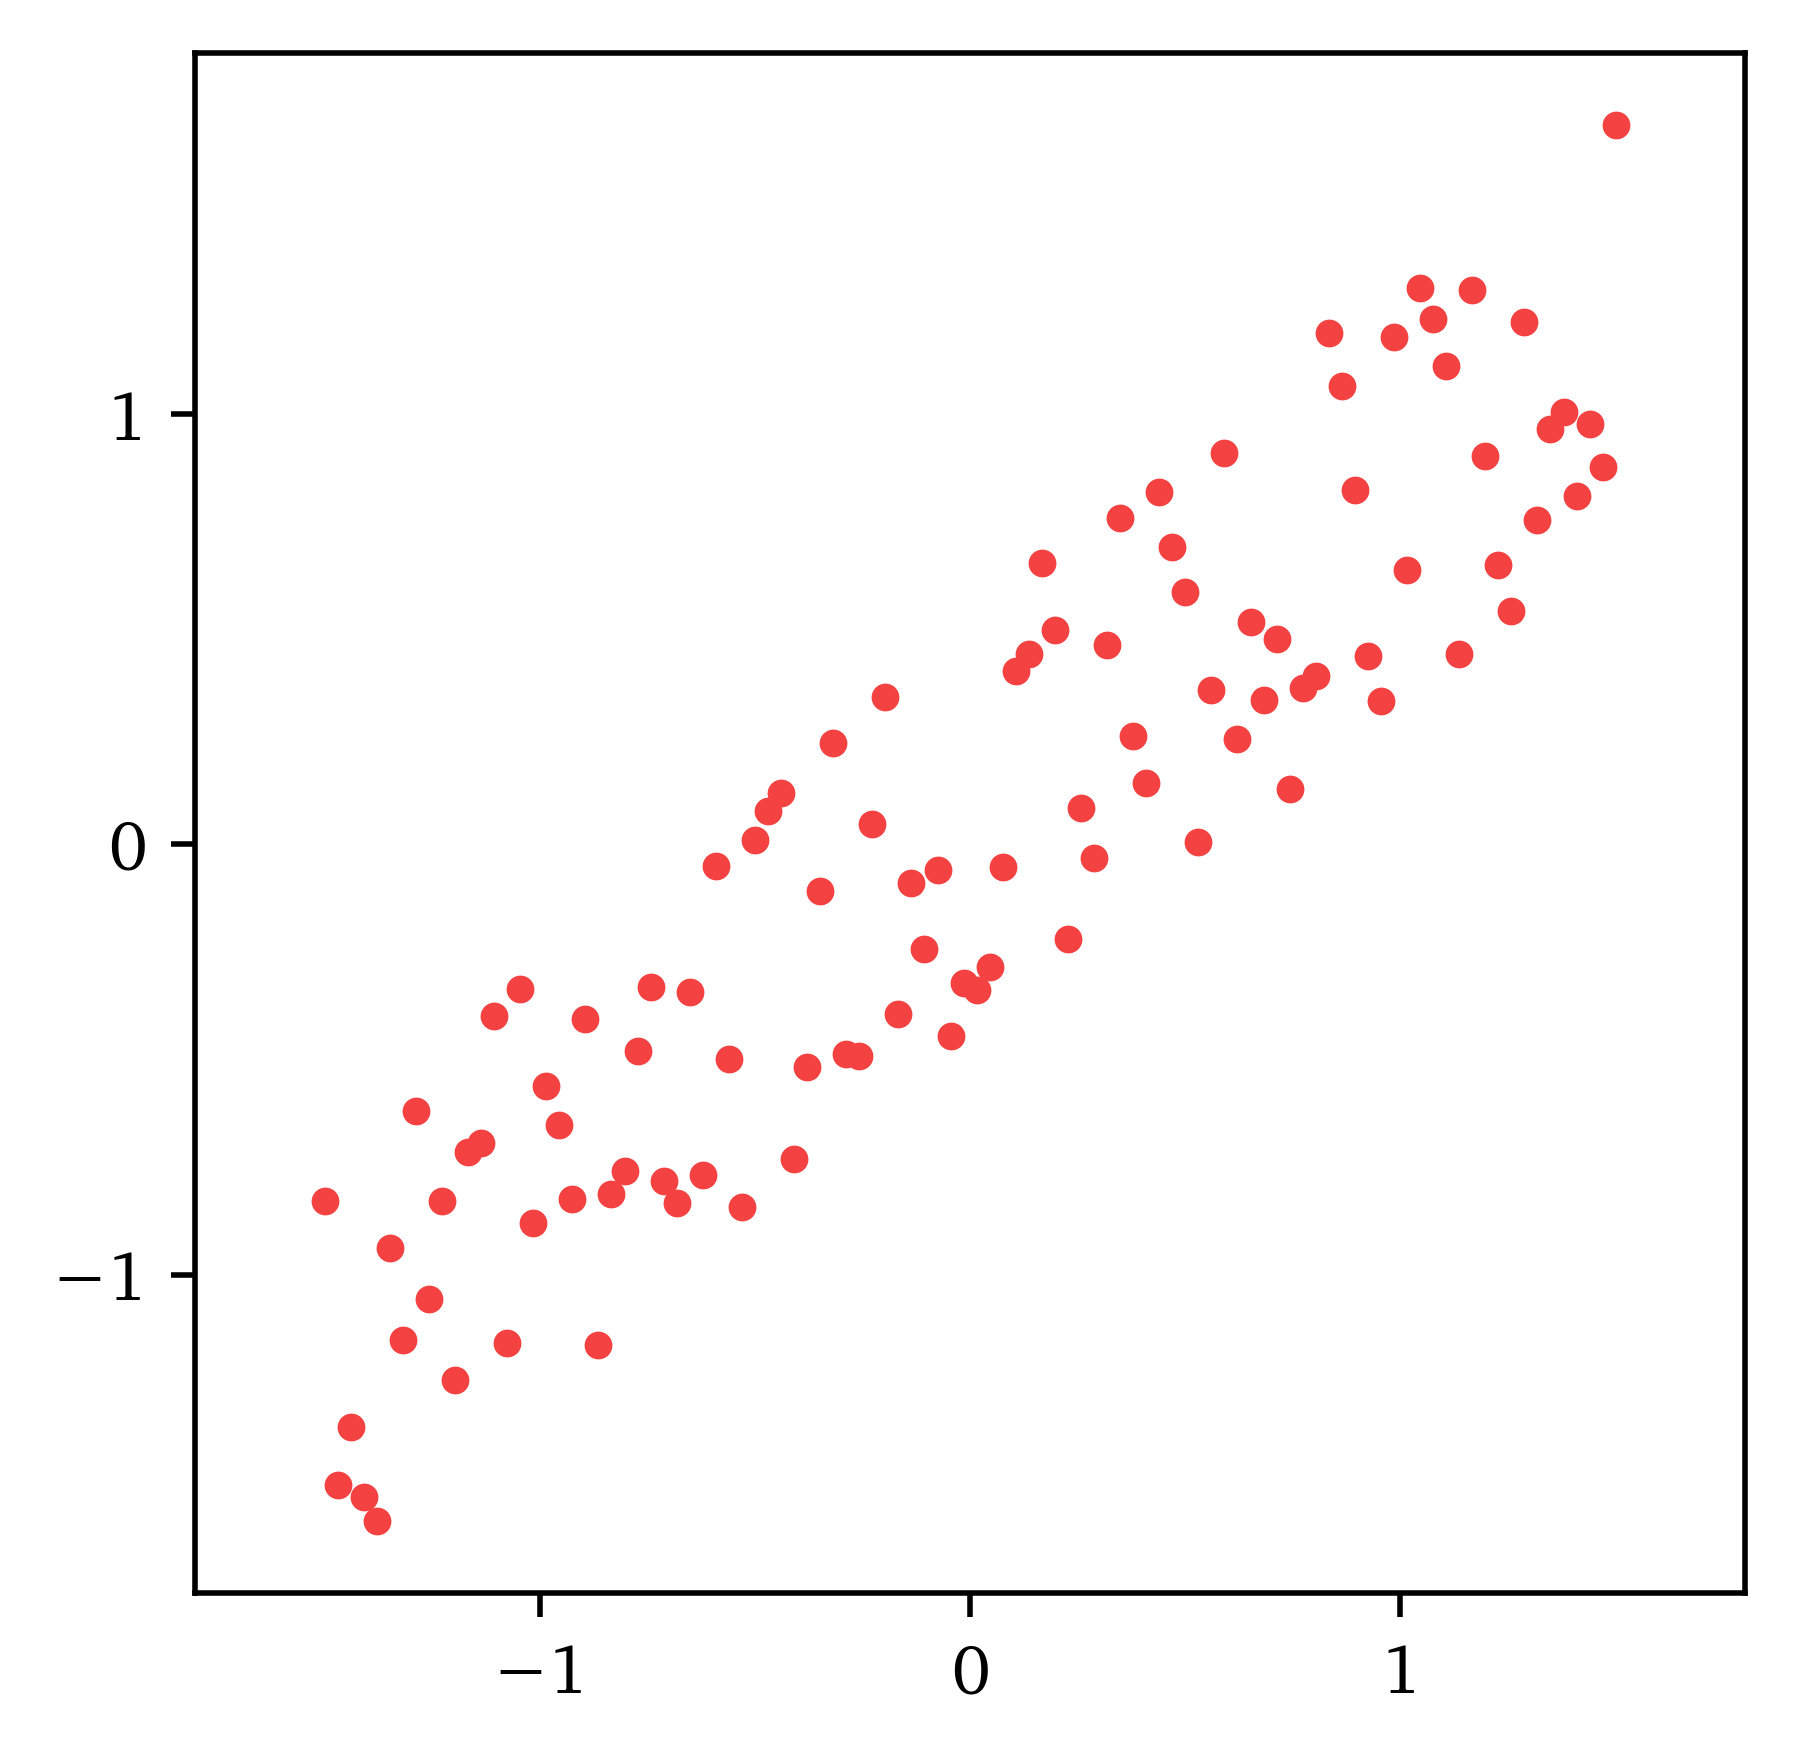
\includegraphics[width=7cm]{python-data-centered.png}
\caption{Data set centered.}
\label{fig:python-raw-data-centered}
\end{figure}

Next, PCA is performed on the dataset and the eigenvectors (the Principal Components) \pythoninline{PCs} are found, with the corresponding eigenvalues \pythoninline{eigvals}.

\begin{python}
from sklearn.decomposition import PCA
pca = PCA(n_components=2)
pca.fit(Dataset)
PCs = pca.components_
eigvals = pca.explained_variance_ratio_
\end{python}

In the above code, we create an object \pythoninline{pca} of class \pythoninline{PCA}. We train the model with our \pythoninline{Dataset} using the \pythoninline{fit} function.

The eigenvectors are plotted on the dataset in Figure \ref{fig:python-PCs}. Their lengths are proportional to their corresponding eigenvalue. Notice that PCA was able to find the direction of the largest variance in the data marked by the direction of the first, longest Principal Component. The second PC is simply perpendicular to the first one.

\begin{figure}[H]
\centering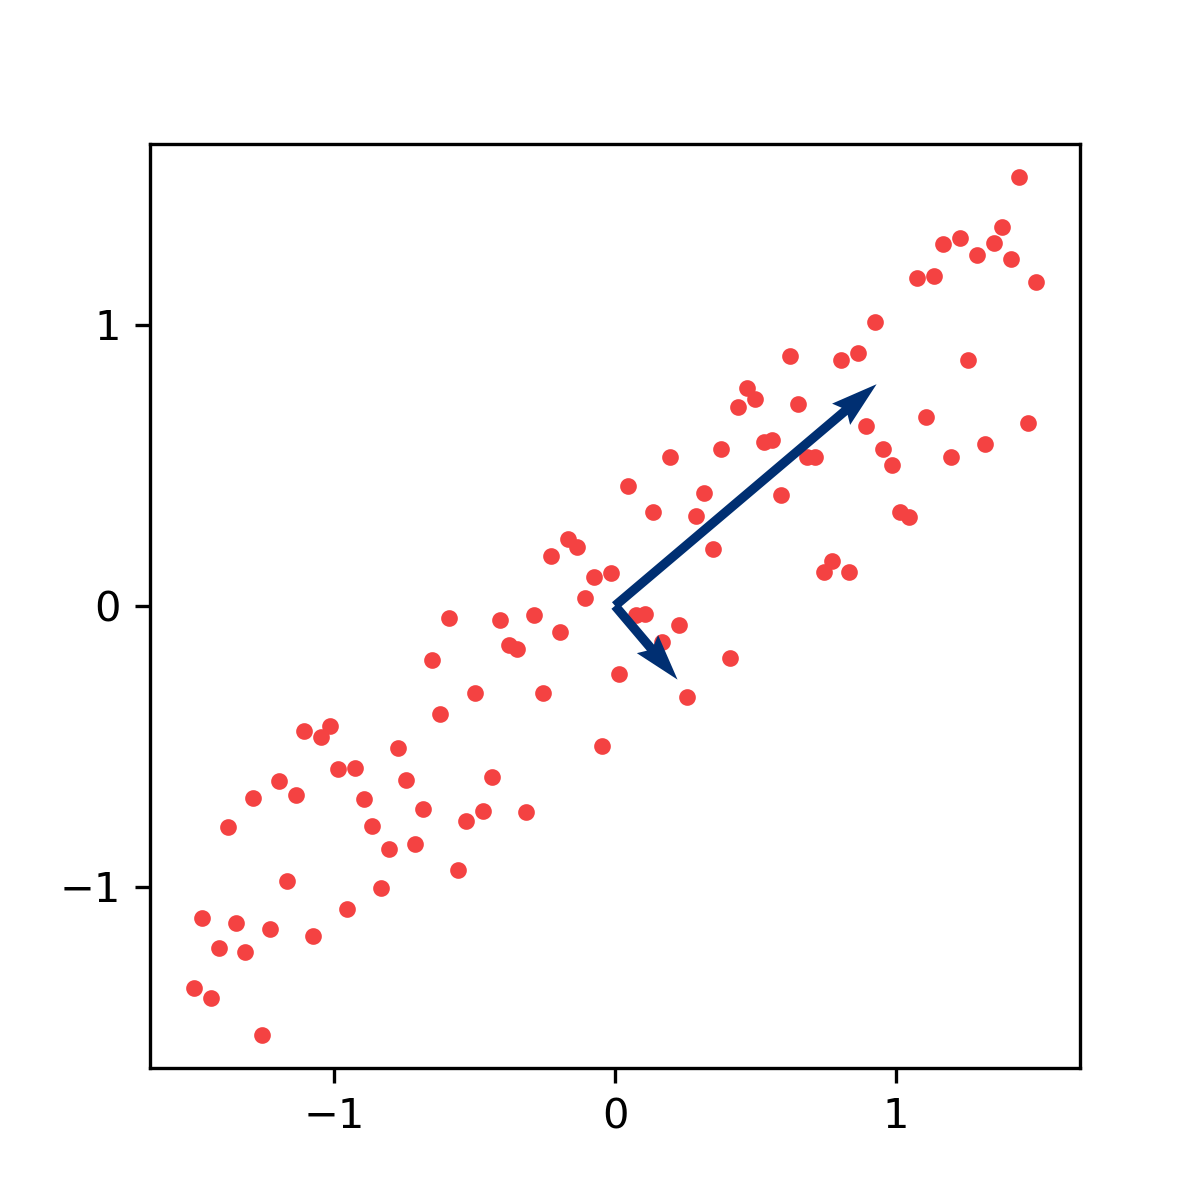
\includegraphics[width=7cm]{python-PCs.png}
\caption{Data set with principal components.}
\label{fig:python-PCs}
\end{figure}

We may now find the PC-scores matrix which represents the "scores" each point from the data set attains when the new coordinate system was associated with the directions of the Principal Components.
 
\begin{python}
scores = pca.transform(Dataset)
\end{python}

\begin{figure}[H]
\centering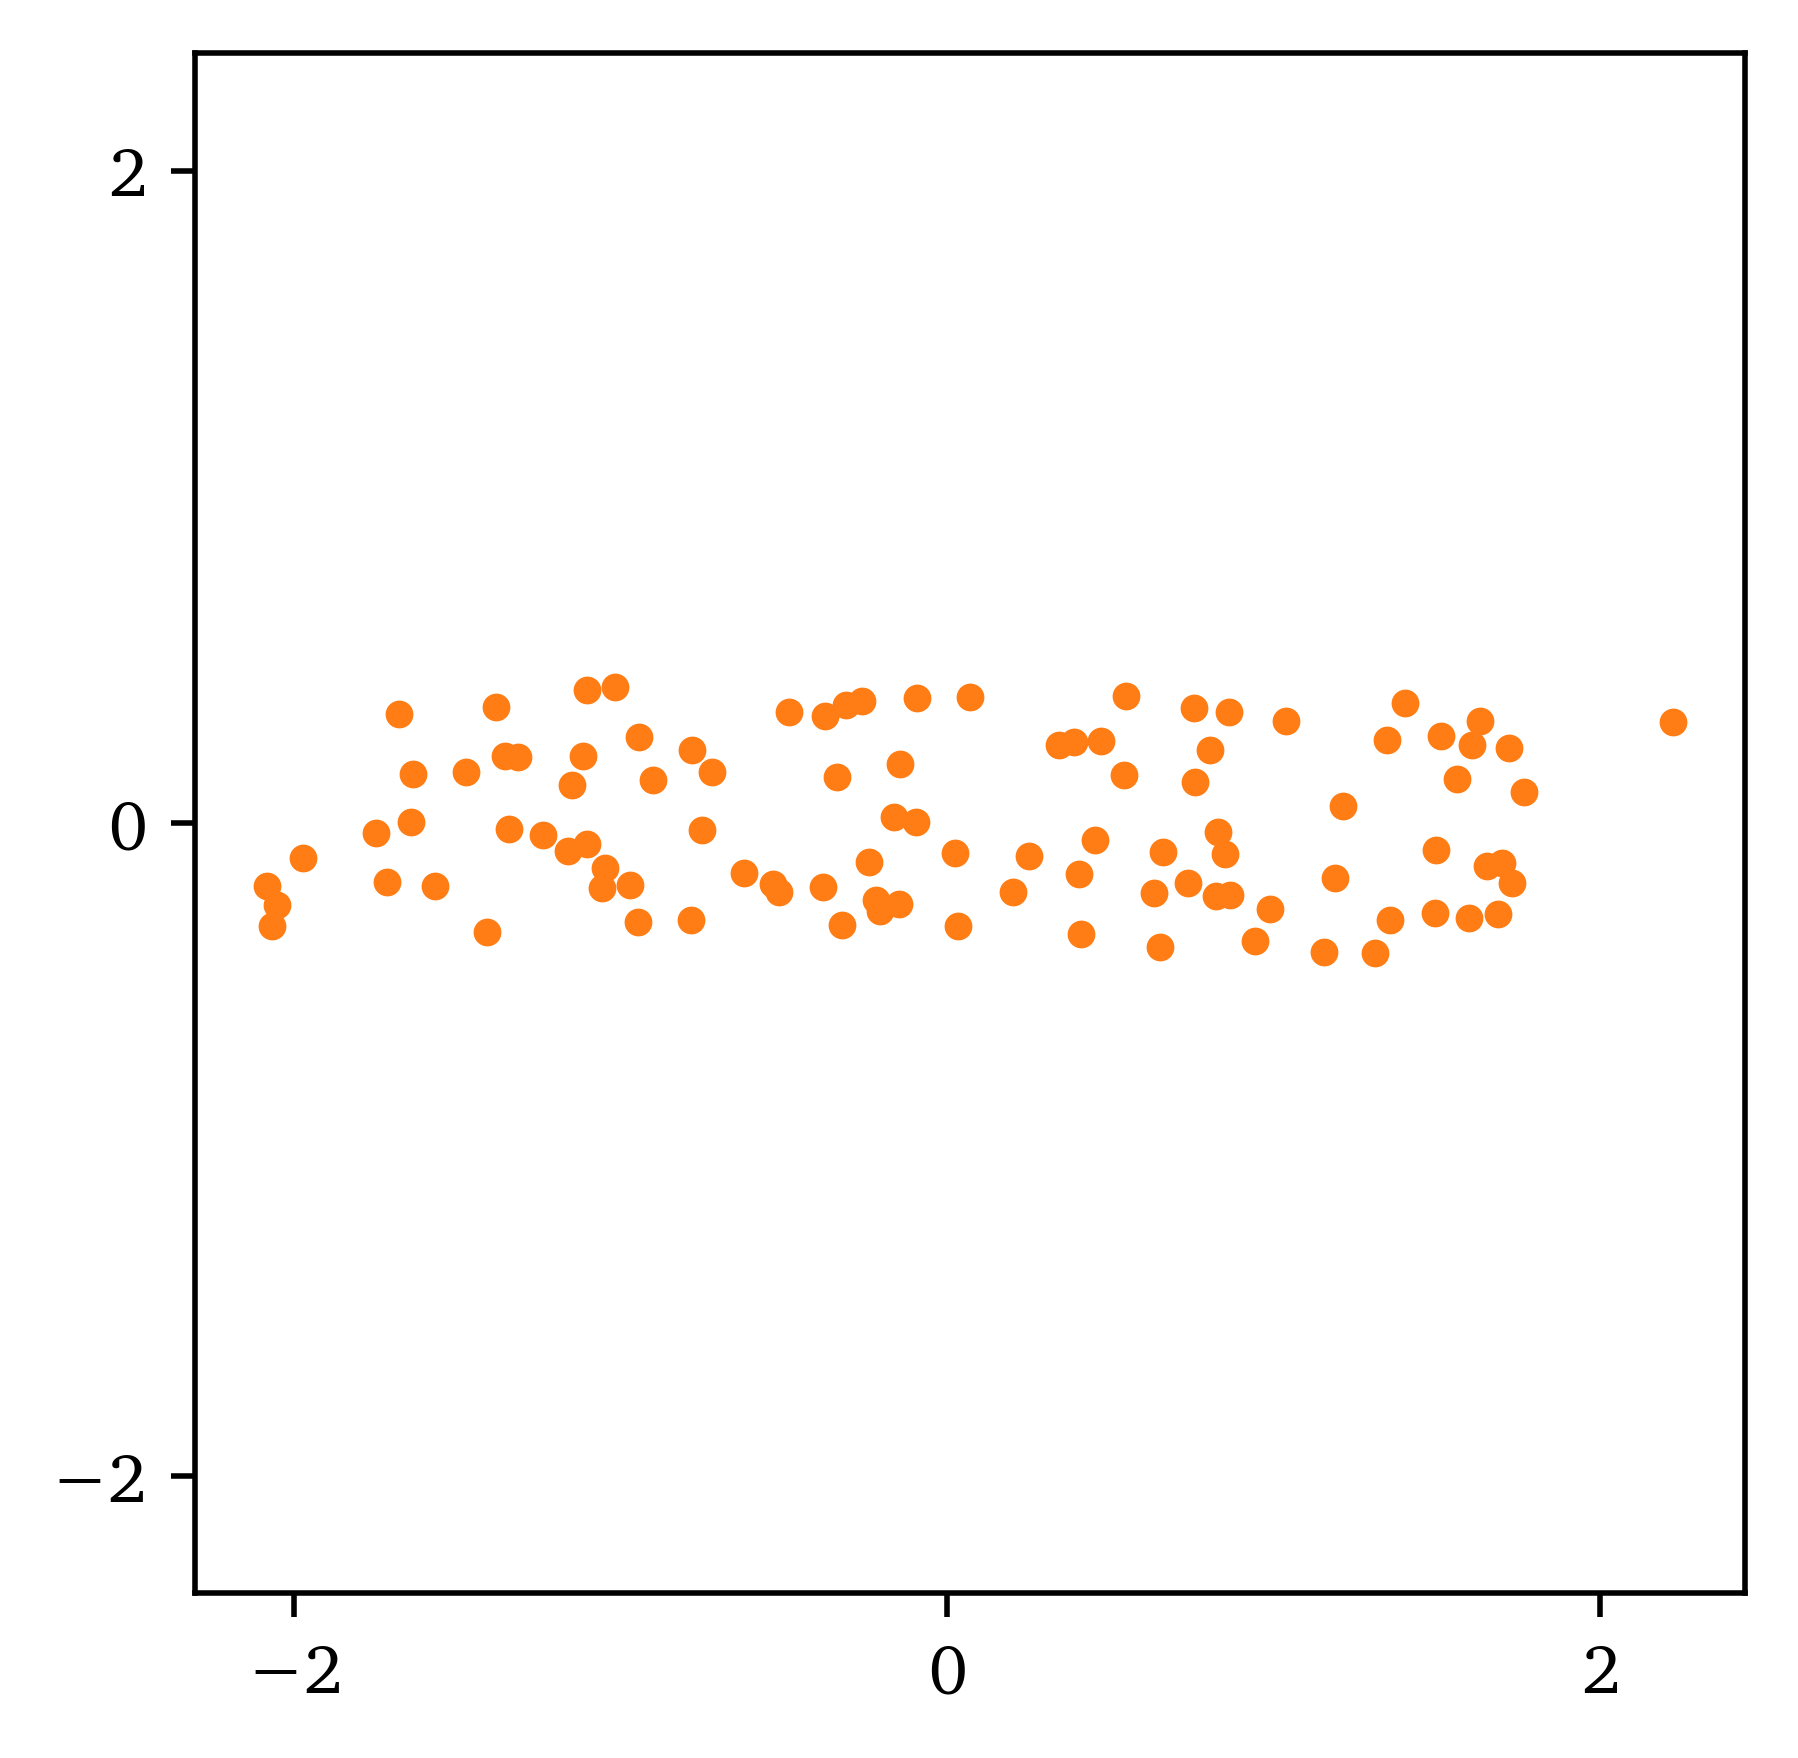
\includegraphics[width=7cm]{python-PC-scores.png}
\caption{PC-scores.}
\label{fig:python-PC-scores}
\end{figure}

Next, the PC-scores can be projected on the first PC, to reduce the dimensionality - from two dimensions to one. The data representation from Figure \ref{fig:python-data-projection} can be viewed as the "scores" each data point would attain it represented on 1-dimensional structure associated with the first Principal Component.

\begin{figure}[H]
\centering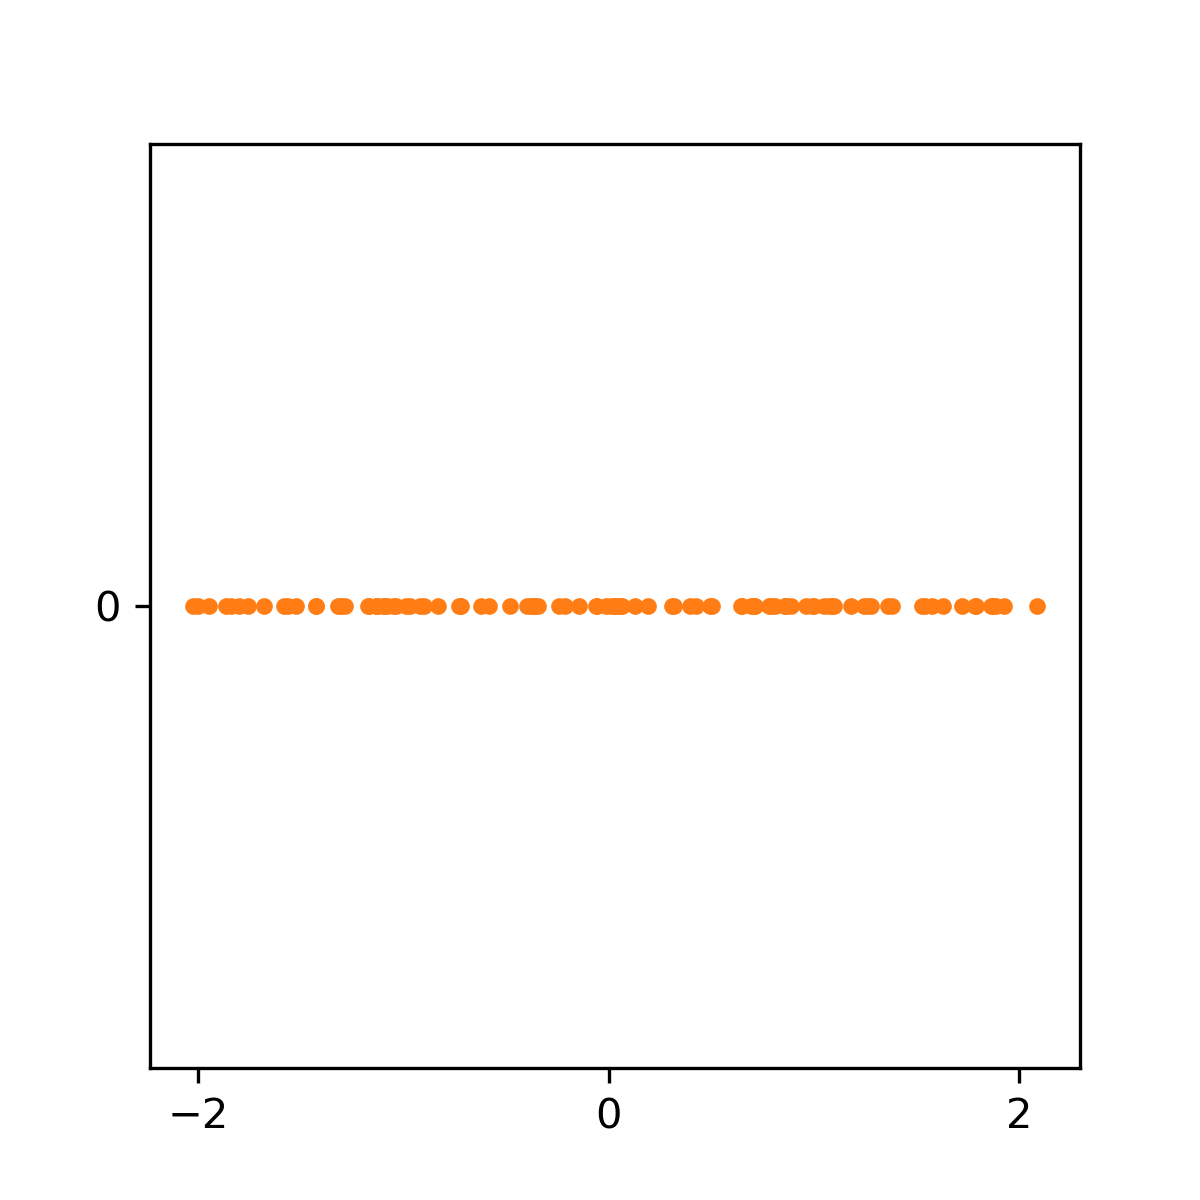
\includegraphics[width=7cm]{python-data-projection.png}
\caption{Data projection on low dimension.}
\label{fig:python-data-projection}
\end{figure}

The data set can be reconstructed. This represents going back from the 1-dimensional space to the original dimensions. The mean of the data set is added back to undo the data centering.

\begin{figure}[H]
\centering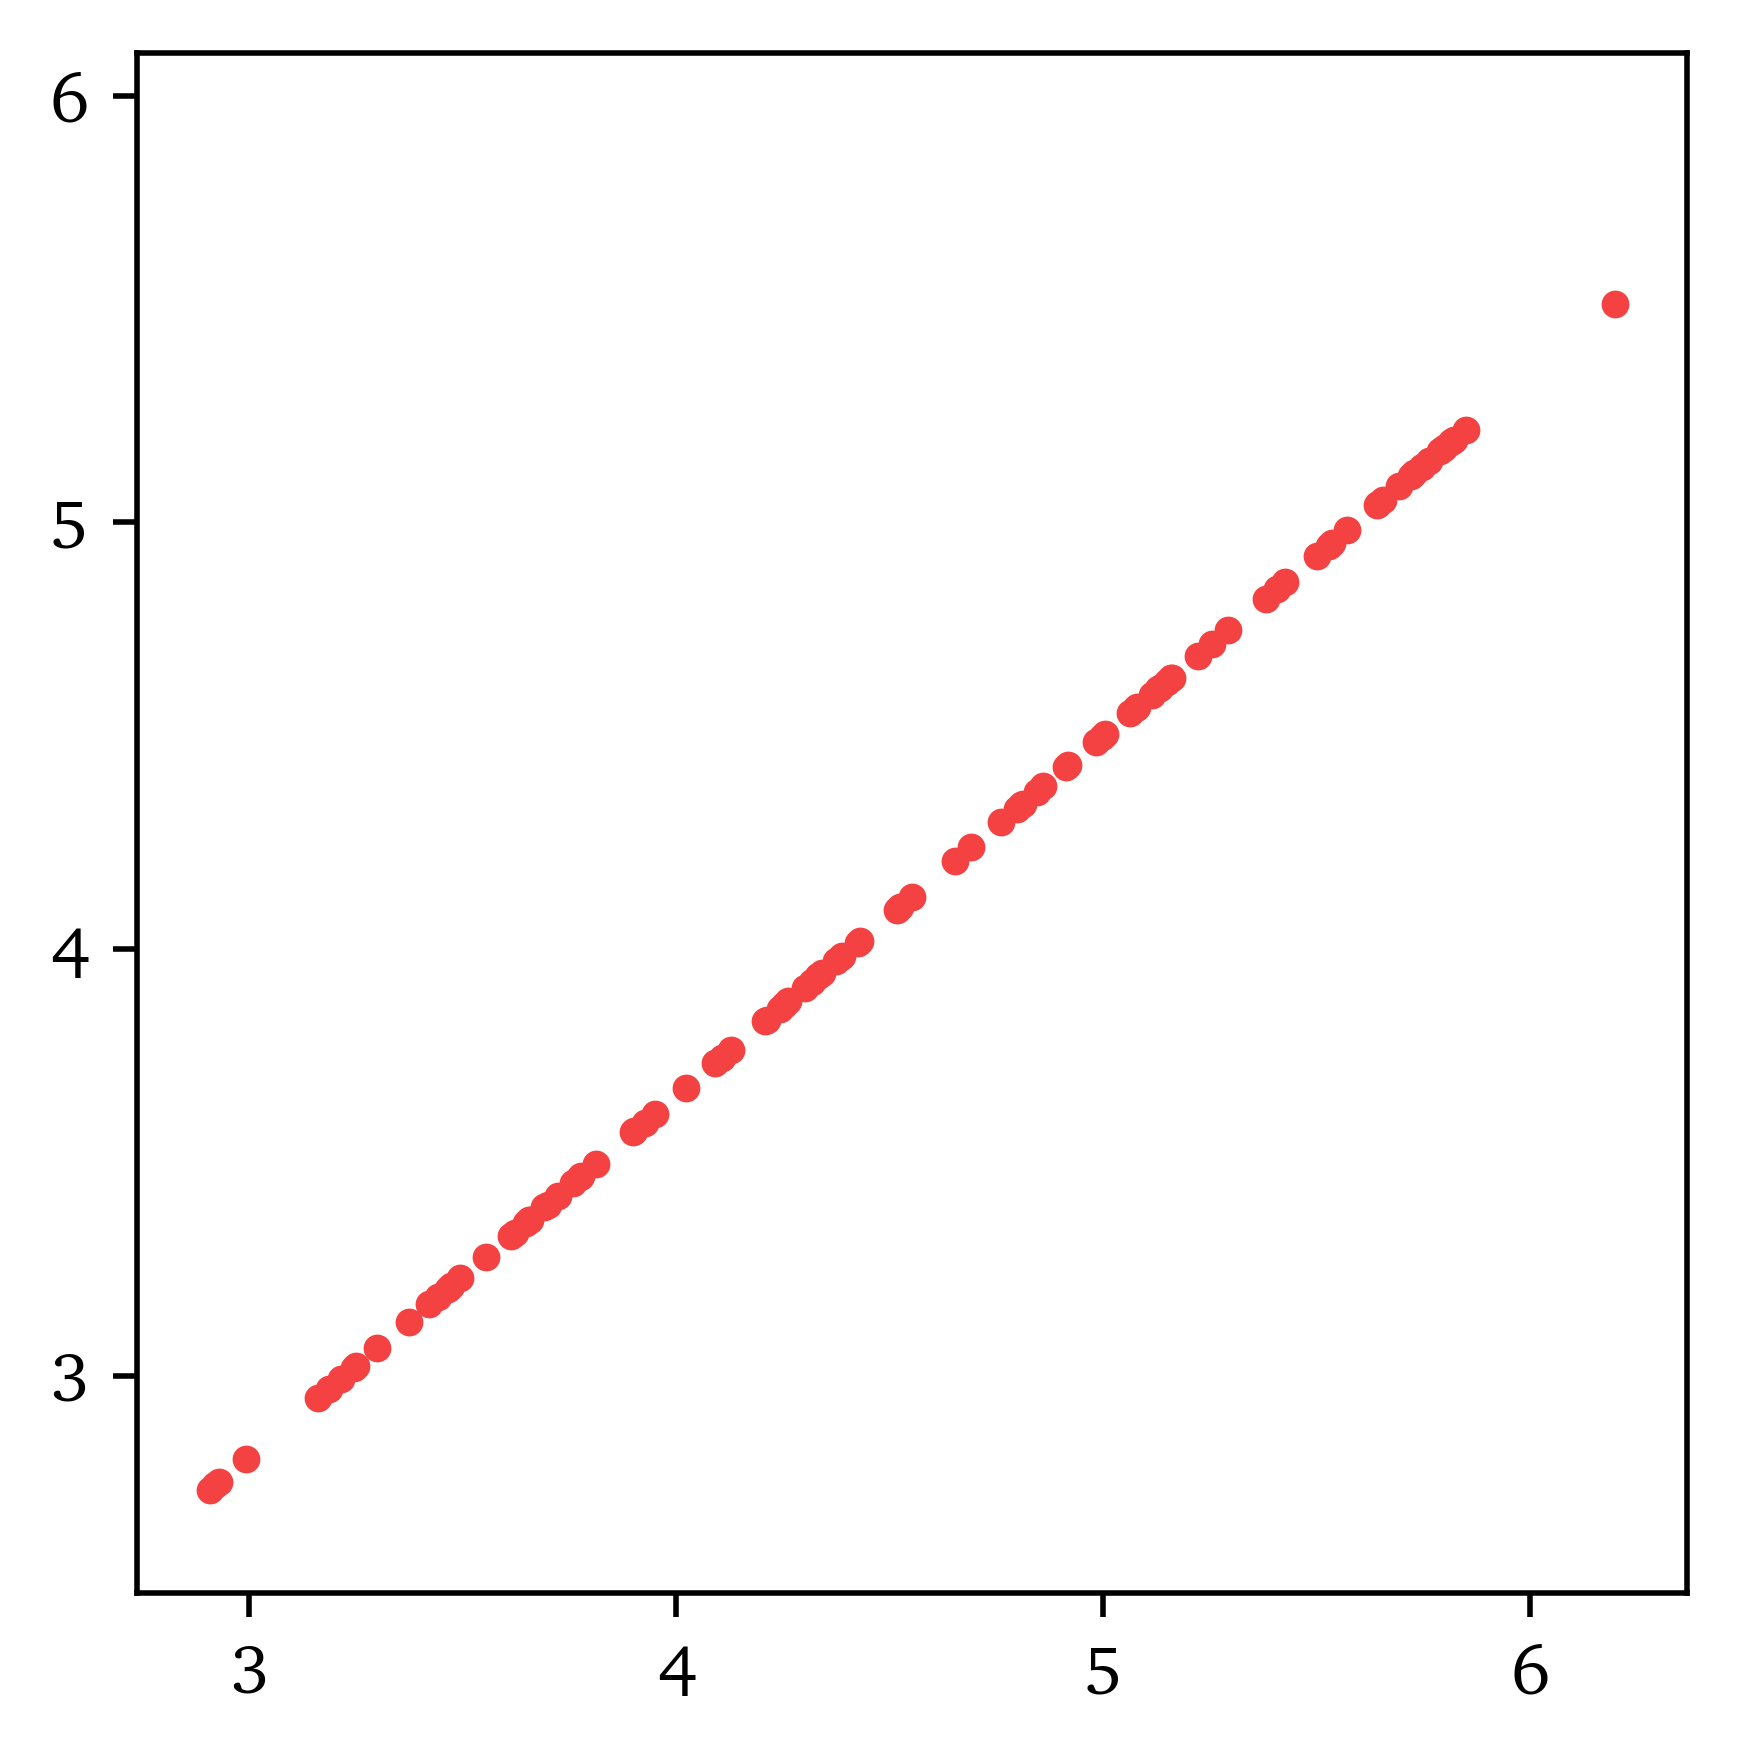
\includegraphics[width=7cm]{python-data-approximation.png}
\caption{Data approximation with $q = 1$.}
\label{fig:python-data-approximation}
\end{figure}

\newpage

\section{Another look, or how it all links together}

\begin{figure}[H]
\centering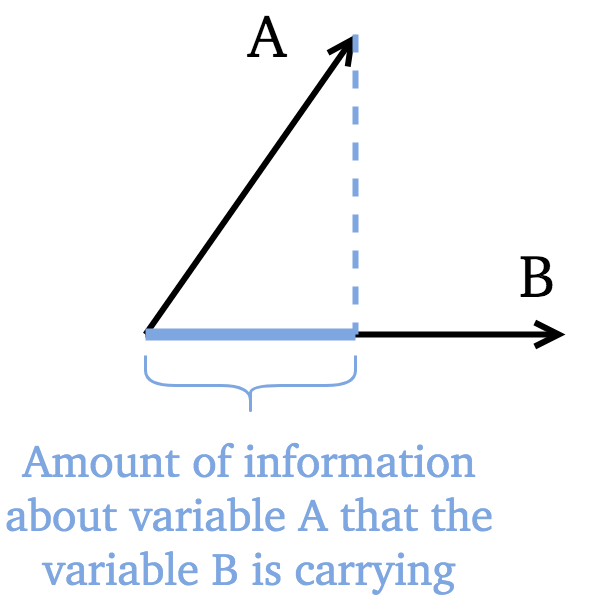
\includegraphics[width=4cm]{variable-basis.png}
\caption{Variable basis might not be optimal.}
\label{fig:variable-basis}
\end{figure}

\begin{figure}[H]
\centering
\includegraphics[width=4cm]{PC-basis.png}
\caption{PC-basis is orthogonal.}
\label{fig:PC-basis}
\end{figure}

\section{Interesting questions}

\subsection{Is the covariance matrix of PC-scores a diagonal matrix?}

\textbf{The goal of PCA in terms of a covariance matrix}

\,\,
\,\,

Principal Component Analysis aims to find a new, transformed data set $\bm{Z}$ such that if we computed a new covariance matrix:

\begin{equation}
\bm{S}_Z =  \bm{Z^T} \bm{Z}
\end{equation}

the variances (the elements on the diagonal) are maximized and the covariances (the off-diagonal elements) are zero. This means that no more information about any column of $\bm{Z}$ is carried by any other column of $\bm{Z}$.

\begin{figure}[H]
\centering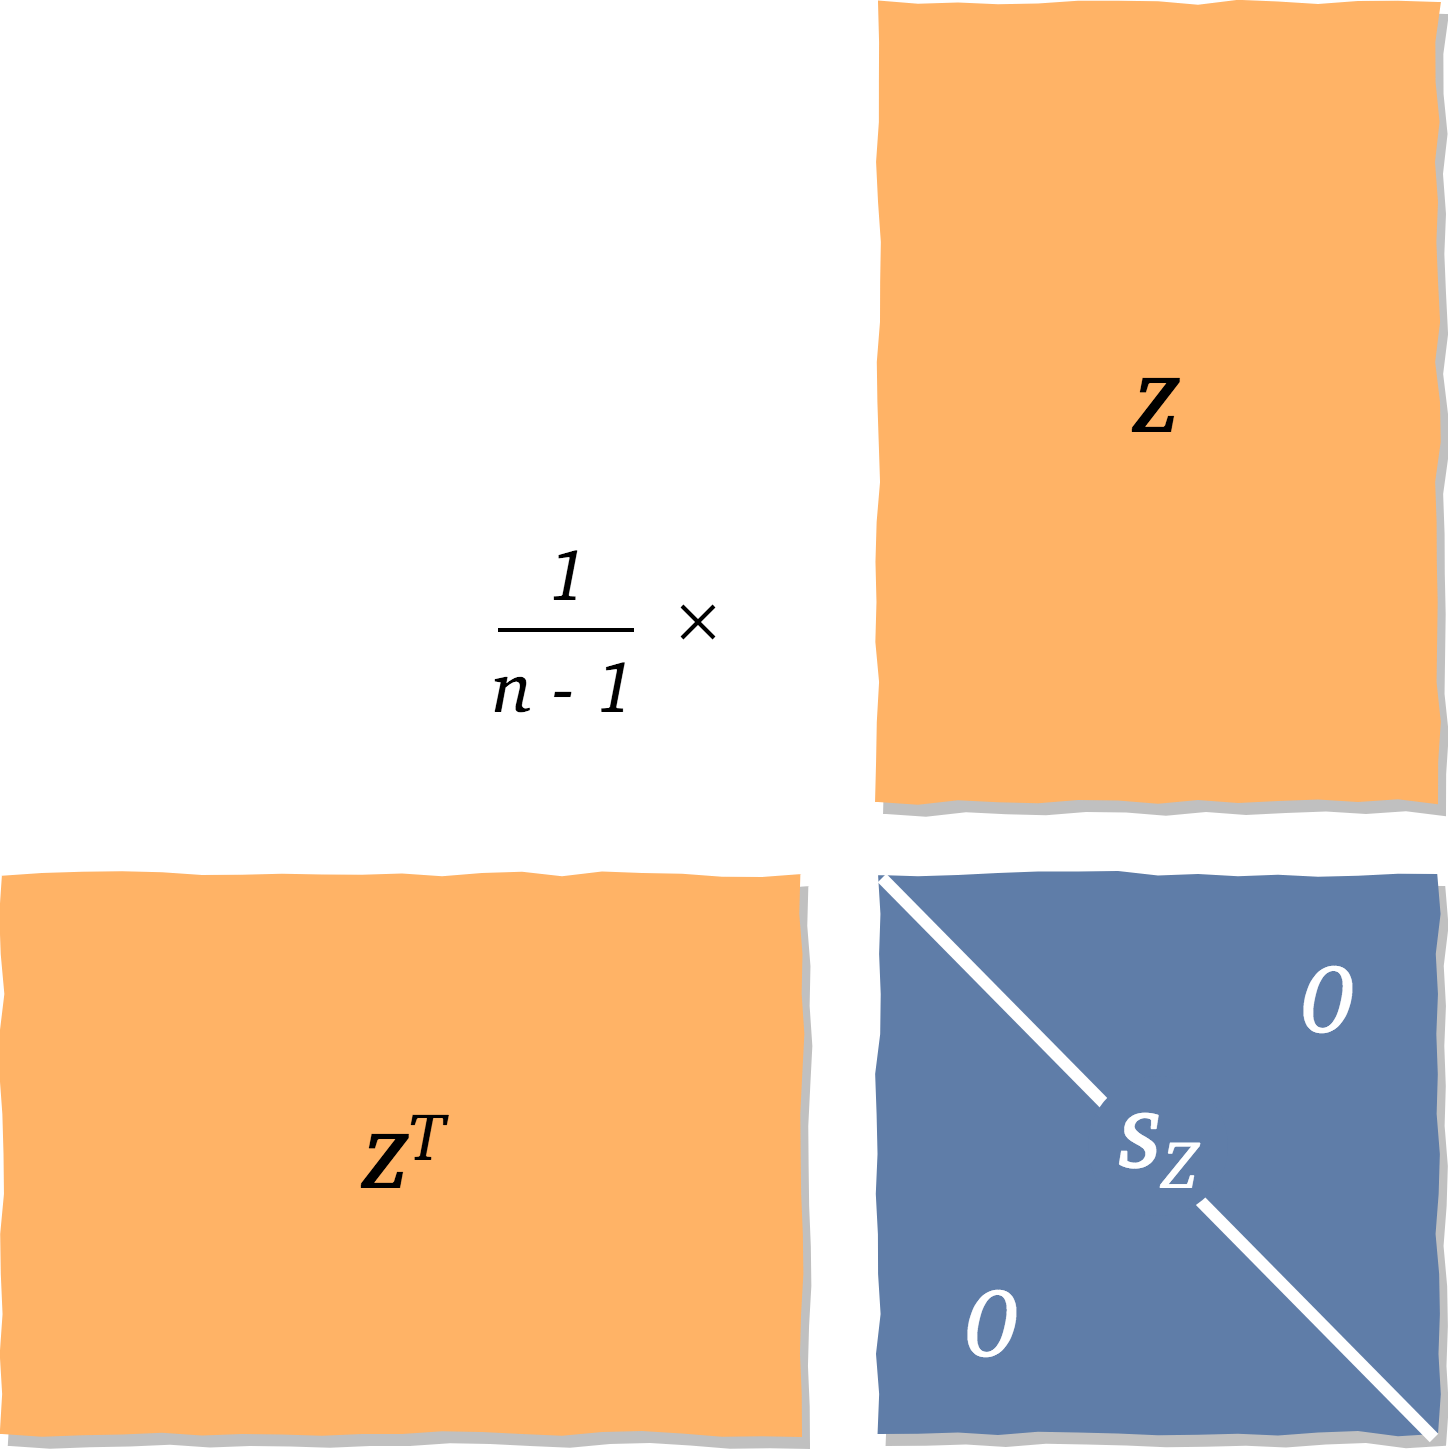
\includegraphics[width=5cm]{PC-scores.png}
\caption{New transformed data set $\bm{Z}$ and its covariance matrix $\bm{S}_Z$.}
\label{fig:PC-scores}
\end{figure}

\appendix

\section{Properties of interesting matrices}

\subsection{Symmetric matrices} \label{app:A}

The properties of symmetric matrices:

\begin{enumerate}
\item Their eigenvectors are orthogonal.
\item Their eigenvalues are real.
\end{enumerate}



\section{Highlights of statistics} \label{app:B}

The intuition behind $\frac{1}{1-n}$.

\thebibliography{}

\bibitem{Matlab-pca} \texttt{https://nl.mathworks.com/help/stats/pca.html}
\bibitem{Jolliffe} Ian T. Jolliffe, \textit{Principal Component Analysis}, Second Edition, 1986
\bibitem{Strang} Gilbert Strang, \textit{Introduction to Linear Algebra}, Fifth Edition, 2016
\bibitem{Shlens} Jonathon Shlens, \textit{A Tutorial on Principal Component Analysis}, 2016, \texttt{https://arxiv.org/abs/1404.1100}
\bibitem{cov-dot} \texttt{http://people.sju.edu/~pklingsb/dot.cov.pdf}
\bibitem{Jackson} J. Edward Jackson, \textit{A User's Guide To Principal Components}, 1991
\bibitem{Smith} Lindsay I. Smith, \textit{A tutorial on Principal Component Analysis}, 2002

\end{document}
